\section{Ancestry and Classes}
\label{Section_AncestryAndClasses}

\textbf{Ancestry} - 
In \textit{Wheel of Elements}, there are 10 different ancestries to choose from. The ancestries are dedicated to \textbf{one Boon or Bane} and often also to an element. Try experimenting to see which playstyles you like. Each ancestry comes with 7 attack dice, one passive, 6 action cards and a tableau.

\textbf{Ancestry Tableau} - Your core tool for tracking character progress.
It contains the ancestry name, places for all of the class tiles, your first passive, a place to track your life, and an overview of the combat turn.


\textbf{Attack Dice} - Take the two dice with the corresponding ancestry icon at the start of the game.


\begin{figure}[ht]
	\centering
	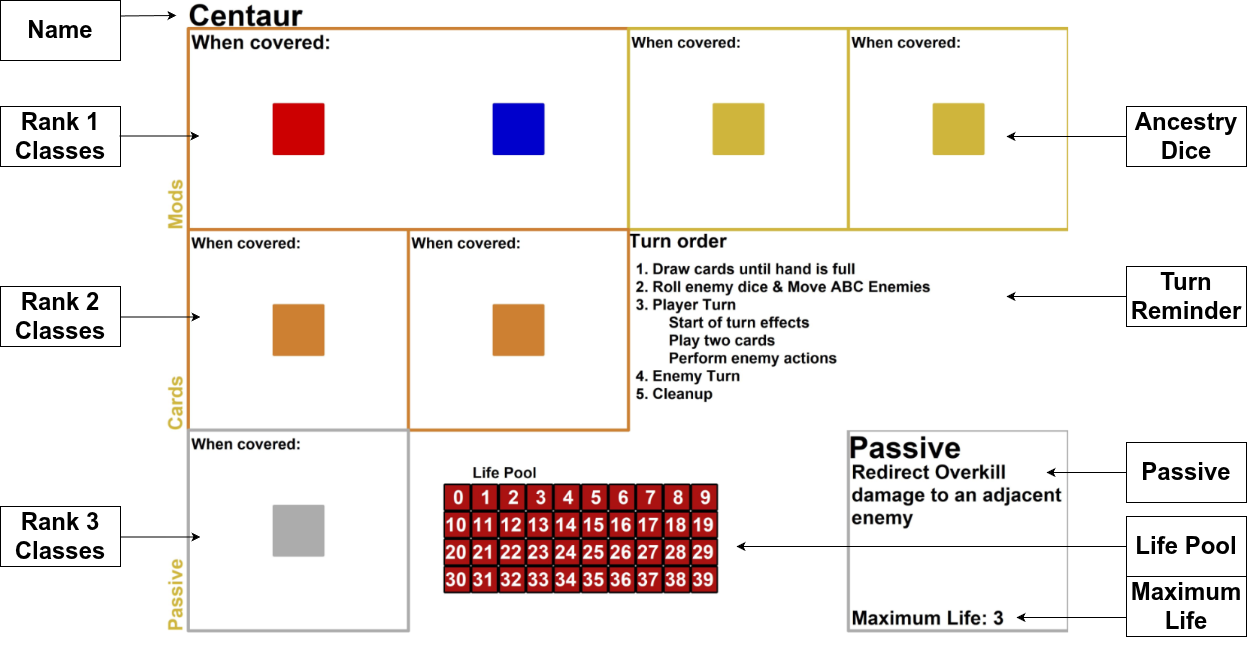
\includegraphics[width=0.9\linewidth, valign=t]{../ExplanationPics/TableauRows.drawio.png}
	
\end{figure}



\begin{figure}[ht]
	\begin{minipage}[t][4.8cm][t]{0.5\textwidth}
		\textbf{Class} - You can chose from 10 different classes during the game. The classes always use \textbf{one or more elements}, as well as \textbf{up to three boons \& banes}. Each class comes with one class tile and 5 action cards. Classes are separated into three ranks. To begin the game, you will choose two rank 1 classes.\\
		\textbf{Rank 1} classes have the \textbf{best cards}, and will allow for compressed powerful turns as you draw those cards.\\
		\textbf{Rank 2} classes emphasise \textbf{best passives} passives to shape your gameplay. 
	\end{minipage}
	\begin{minipage}[t][4.8cm][t]{0.5\textwidth}
		\centering
		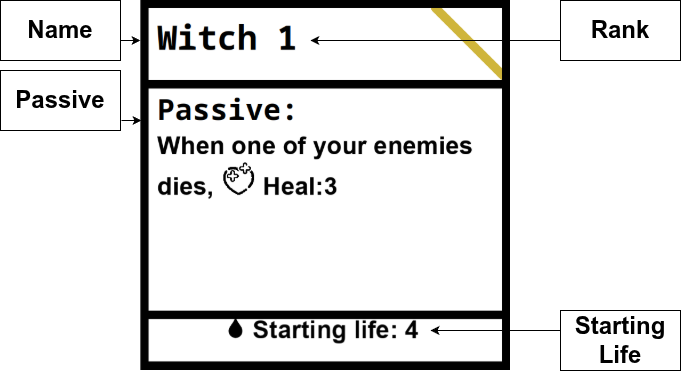
\includegraphics[width=0.9\linewidth, valign=t]{../ExplanationPics/ClassShingle.drawio.png}
	\end{minipage}
\end{figure}

\textbf{Passives} - The passives you acquire will shape your gameplay immensely. Passives come in three varieties: 

\begin{itemize}
	\item \textbf{Trigger} - These passives apply at specific times, like the start of combat, or the end of your turn. You are granted a concrete benefit at the specified time.
	\item \textbf{Permanent} - Some passives modify the way you perform actions permanently. For example, you might gain the ability to use your ancestry dice when applying certain Boons or Banes.
	\item \textbf{Shaping} - Some passives modify what you would normally get from an ancestry or class. They might provide additional ancestry dice, more powerful cards, or simply more maximum life.
\end{itemize}

\begin{tcolorbox}[colframe=blue, colback=white]
	Reminder -	The tableau provides a helpful overview of all of the passives that affect you.
\end{tcolorbox}